\begin{figure*}[t]
\centering
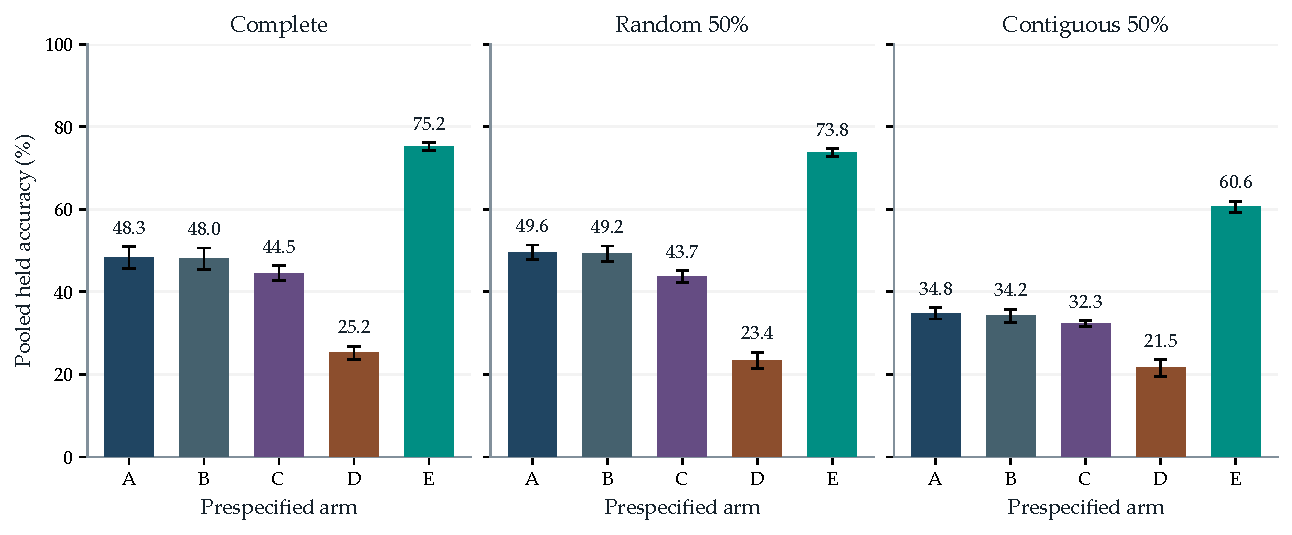
\includegraphics[width=.98\textwidth]{mira_v2_held_accuracy.pdf}
\caption{Every prespecified arm on pooled held recordings. Error bars are sample SD over five training seeds, after averaging masks within seed; they are not confidence intervals. Complete input uses one realization. Random and contiguous loss each remove 250 normalized positions shared by all channels. The feature-only arm E performs substantially better here than the hybrid arms; the plot retains the unsuccessful main candidate A and temporal control D.}
\label{fig:m2-held}
\end{figure*}
\begin{figure*}[t]
\centering
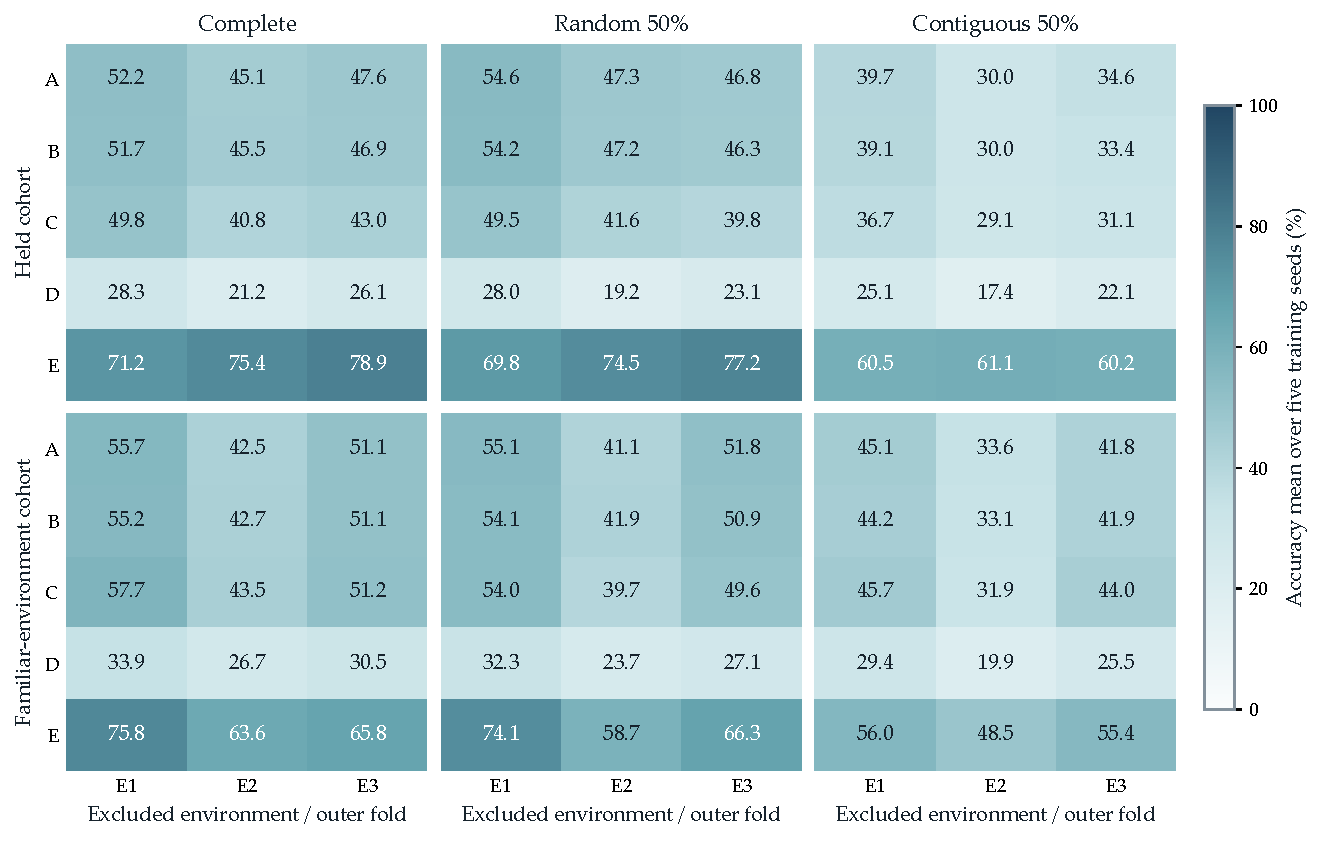
\includegraphics[width=.98\textwidth]{mira_v2_fold_domain_accuracy.pdf}
\caption{All arms, folds and cohort domains. Each cell shows mean accuracy across five training seeds after mask averaging, on a common 0--100\% colour scale. Top: the excluded environment/cohort; bottom: participants held out within the remaining two environments. E1--E3 always identify the excluded environment. Familiar and held scores are not mixed, and familiar scores are not consistently greater. Full sample SD, macro F1, NLL and Brier appear in Supplementary Tables S1--S6; Table~\ref{tab:m2-E} retains E's full 18-row breakdown in the main text.}
\label{fig:m2-folds}
\end{figure*}
\begin{figure*}[t]
\centering
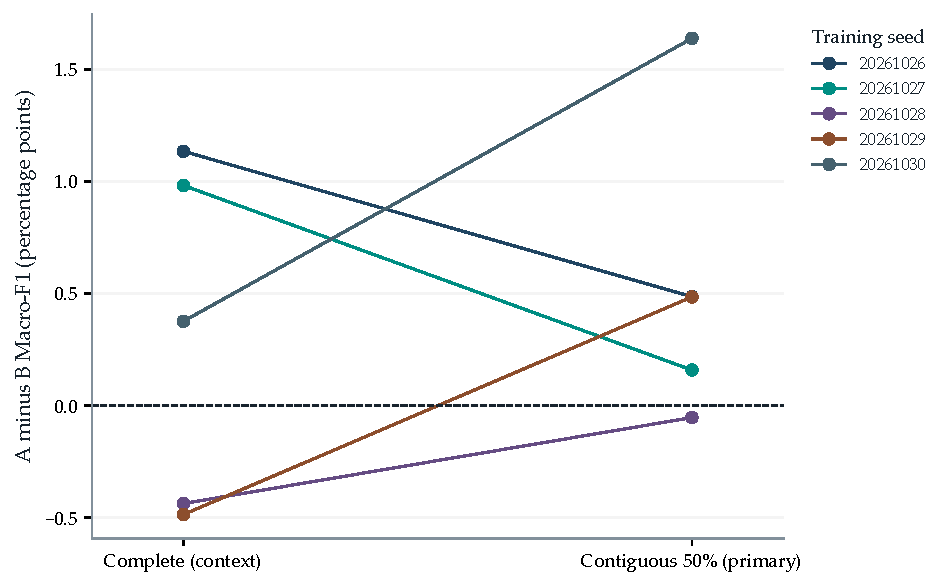
\includegraphics[width=.78\textwidth]{mira_v2_primary_paired_contrast.pdf}
\caption{Paired A minus B macro-F1 differences for each training seed. Loss-mask results are averaged before forming the five seed differences. The primary contiguous-loss contrast is $+0.543\pm0.654$ percentage points, with four positive and one negative seed difference. The clean differences are retained as context because A and B also differ on complete input. Lines join the same seed; they do not describe a physical trajectory or independent participant observations.}
\label{fig:m2-primary}
\end{figure*}
